\section{Torsion}

\textbf{Torsion} refers to the twisting of a specimen when it is loaded by couples (or \textbf{moments}) that produce rotation about the longitudinal axis. Applications include aircraft engines, car transmissions, and bicycles, etc.

\subsection{\blue{Units}}

Force X distance [lb-in or N-m]

\subsection{\blue{Notation and Convention}}

\begin{figure*}[!h]
\centering
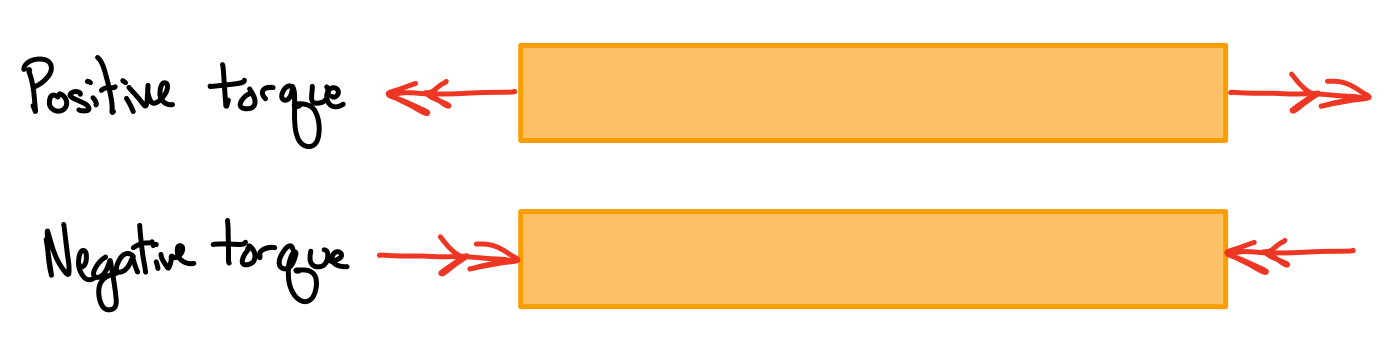
\includegraphics[angle=0, width=5in]{Torsion-Figures/Convention.png}
\vspace{-2mm}
\caption{\small \blue{Taken from TAM251 Lecture Notes - L5S11}}
\vspace{-3mm}
\label{Fig:TorsionConvention}
\end{figure*}

\blue{
\begin{itemize}
    \item $\phi > 0$: counter clockwise 
    \item $\phi < 0$: clockwise
\end{itemize}
}

\begin{figure*}[!h]
\centering
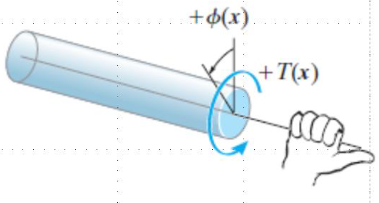
\includegraphics[angle=0, width=2in]{Torsion-Figures/RightHandRule.png}
\vspace{-2mm}
\caption{\small \blue{Taken from TAM251 Lecture Notes - L5S11}}
\vspace{-3mm}
\label{Fig:RHR}
\end{figure*}

\noindent Torque and angle of twist follow the right hand rule sign convention. When positive, using the right hand, the thumb points outward from the shaft and the fingers will curl in the direction of the positive twist/torque.



\subsection{\blue{Equilibrium}}
\blue{
The stress distribution in the shaft is not known.
\begin{itemize}
    \item Statically indeterminate: must consider shaft deformations.
    \item Multi-planar: equilibrium requires the existence of shear stresses on the faces formed by the two planes containing the axis of the shaft
\end{itemize}
}
\begin{figure*}[!h]
\centering
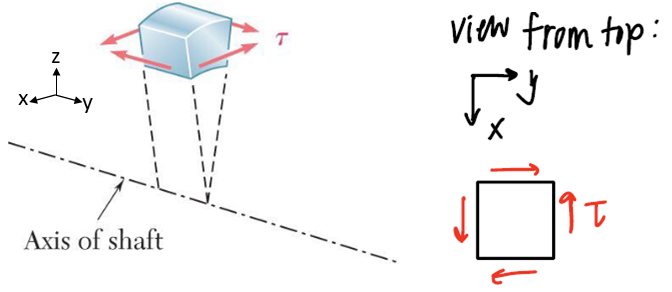
\includegraphics[angle=0, width=4in]{Torsion-Figures/Equilibrium.png}
\vspace{-2mm}
\caption{\small \blue{Taken from TAM251 Lecture Notes - L5S3}}
\vspace{-3mm}
\label{Fig:Equilibrium}
\end{figure*}

\subsection{\blue{Assumptions}}

\begin{itemize}
    \item For circular shafts (hollow and solid): cross-sections remain plane and undistorted due to axisymmetric geometry
    \begin{itemize}
        \item i.e. while different cross sections have distinct angles of twist, each one of them rotates as a solid rigid slab
        \item Longitudinal lines twist into a helix that intersects the circular cross sections at equal angles
    \end{itemize}
    \item For non-circular shafts,: cross-sections are distorted when subject to torsion
    \begin{itemize}
        \item Cross-sections warp and do not remain plane
    \end{itemize}
    \item Linear and elastic deformation
\end{itemize}

\begin{figure*}[!h]
\centering
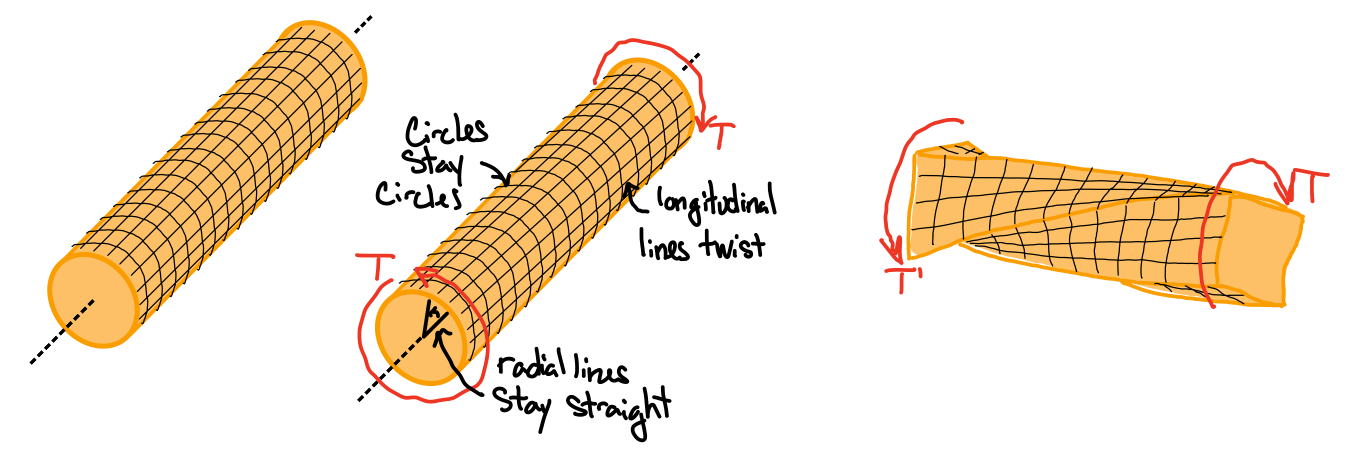
\includegraphics[angle=0, width=6in]{Torsion-Figures/TorsionLines.png}
\vspace{-2mm}
\caption{\small \blue{Taken from TAM251 Lecture Notes - L5S5}}
\vspace{-3mm}
\label{Fig:Lines}
\end{figure*}

\subsection{\blue{Shear Stress and Strain}}

\subsubsection{\blue{Shear Strain: Geometry of Deformation}}

\begin{figure*}[!h]
\centering
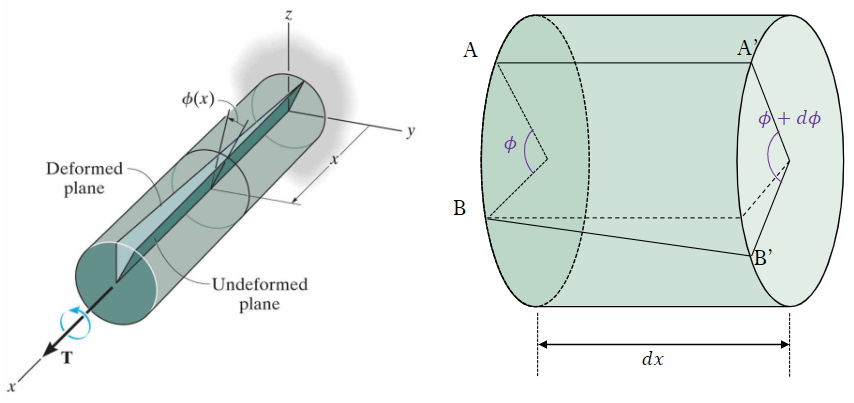
\includegraphics[angle=0, width=4in]{Torsion-Figures/GeometryDeformation.png}
\vspace{-2mm}
\caption{\small \blue{Taken from TAM251 Lecture Notes - L5S6}}
\vspace{-3mm}
\label{Fig:Lines}
\end{figure*}

\noindent The angle of twist increases as x increases. The twist rate is given by: \[\frac{d\phi}{dx} = \frac{\gamma}{\rho} = \frac{\gamma_{max}}{c}\]

\noindent Moving terms we get:\[\gamma = \rho \frac{d\phi}{dx}\]

\noindent Hence, the shear strain ($\gamma$):
\begin{itemize}
    \item is proportional to the angle of twist
    \item varies linearly with the distance from the axis of the shaft
    \item is \textbf{maximum} at the surface
\end{itemize}

\subsubsection{\blue{Shear Stress: Torsion Formula}}

Geometry: \[\gamma = \rho \frac{d\phi}{dx}\]

\noindent Hooke's Law: \[\tau = G\gamma\]

\noindent From equilibrium: \[\frac{d\phi}{dx} = \frac{T}{GJ}\]

\noindent Elastic torsion formula: \[\tau = \frac{T\rho}{J}\]

\noindent \blue{The shear stress in the elastic range varies linearly with the radial position in the section}

\begin{figure*}[!h]
\centering
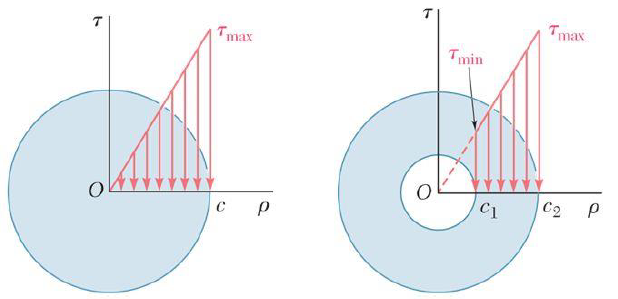
\includegraphics[angle=0, width=4in]{Torsion-Figures/StressDistribution.png}
\vspace{-2mm}
\caption{\small \blue{Taken from TAM251 Lecture Notes - L5S8}}
\vspace{-3mm}
\label{Fig:StressDist}
\end{figure*}

\noindent \blue{\textit{Note:} shaft under torque T rotating at angular speed w transmits power  
\[P=T\omega\]}

\subsubsection{Shear Stress: Polar Moment of Inertia}

Solid Shaft (radius and diameter): \[J = \int_0^R{\rho^2dA} = \int_0^R{\rho^2(2\pi\rho d\rho)dA} =2\pi \int_0^R{\rho^3d\rho} = \frac{\pi R^4}{2} = \frac{\pi D^4}{32}\]

\noindent Hollow Shaft (inner and outer radius): \[J = \frac{\pi}{2}(R_o^4-R_i^4) = \frac{\pi}{32}(D_o^4-D_i^4)\]

\subsubsection{\red{Shear Stress: Symmetry in Axial Planes-?? \cyan{BSM: not sure what this topic is; can probably omit}}}

\noindent \textbf{\red{**Reference pages have a broken link image X2 here and no text**}}

\subsubsection{Shear Stress: Angle of Twist}
From observation:
\begin{itemize}
    \item The angle of twist of the shaft is proportional to the applied torque $\phi \propto T$
    \item The angle of twist of the shaft is proportional to the length $\phi \propto L$
    \item The angle of twist of the shaft decreases when the diameter of the shaft increases
\end{itemize}


\noindent \textbf{Angle of Twist:} \[\phi = \frac{TL}{GJ}\]

\noindent Torsional stiffness: \[k_T = \frac{GJ}{L}\]

\noindent Torsional flexibility: \[f_T = \frac{L}{GJ}\]


\subsection{Miscellaneous}
\subsubsection{Types of Material Failure}

\textbf{Ductile }materials generally fail in shear

\begin{figure*}[!h]
\centering
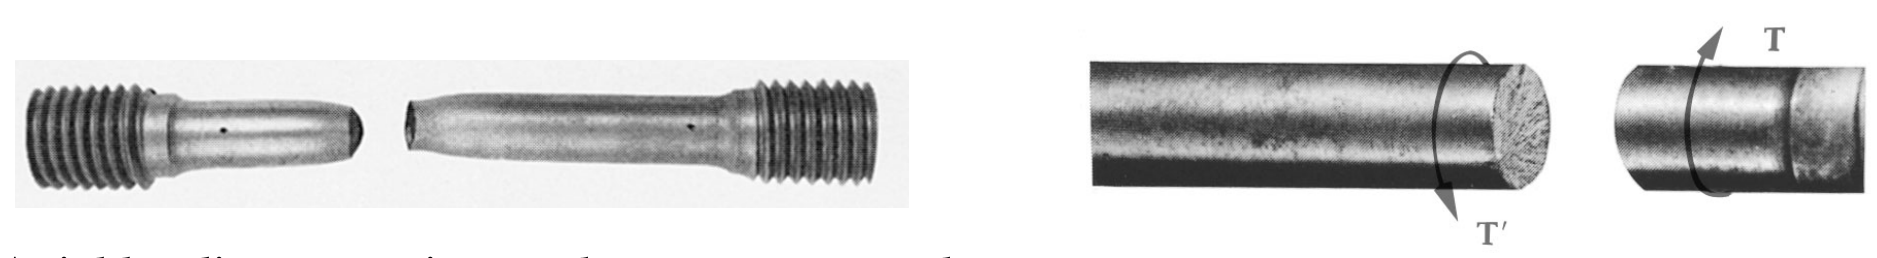
\includegraphics[angle=0, width=4in]{Torsion-Figures/ductile.png}
\vspace{-2mm}
\caption{\small From reference pages}
\vspace{-3mm}
\label{Fig:Ductile}
\end{figure*}

\begin{multicols}{2}
\begin{itemize}
    \item Axial – maximum shear stress at $45^o$ angle
    \item Torsion – maximum shear stress at $0^o$ angle
\end{itemize}
\end{multicols}

 
\noindent \textbf{Brittle} materials are weaker in tension than shear
\begin{figure*}[!h]
\centering
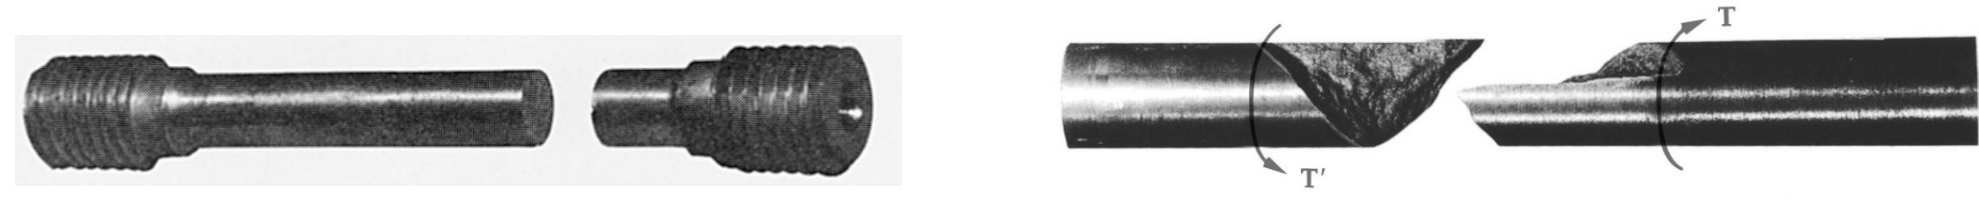
\includegraphics[angle=0, width=4in]{Torsion-Figures/brittle.png}
\vspace{-2mm}
\caption{\small From reference pages}
\vspace{-3mm}
\label{Fig:Brittle}
\end{figure*}

\begin{multicols}{2}
\begin{itemize}
    \item Axial – maximum normal stress at $0^o$ angle
    \item Torsion – maximum normal stress at $45^o$ angle
\end{itemize}
\end{multicols}


\subsubsection{Thin-walled hollow shafts \cyan{BSM: we do not cover this topic in class/hw/exams. Not sure if/when this topic is covered in ME curriculum.}}

In general, the maximum shear stress is given by \[\phi = \frac{TL}{GJ}\]

\noindent For thin-walled shafts: \[\tau_{max} = \frac{T}{2tA_m}\]

\noindent where \[A_m = \pi R_{ave}^2\] \[R_{ave} = \frac{R_o + R_i}{2}\]

\noindent Note that is NOT the cross sectional area of the hollow shaft!



\subsubsection{\blue{Gear Systems - do we want to add?}}

\cyan{BSM: I think it's a nice idea to add some basic info/equations. The biggest is the constraint of the statics version of the ``no slip'' condition between gears (mated gears twist through the same arc length).}


\begin{figure*}[!h]
\centering
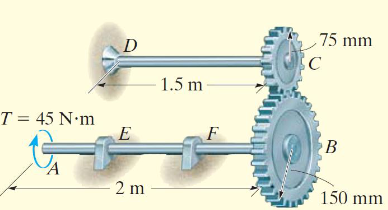
\includegraphics[angle=0, width=3in]{Torsion-Figures/GearSystem.png}
\vspace{-2mm}
\caption{\small \blue{Taken from TAM251 Lecture Notes - L5S15}}
\vspace{-3mm}
\label{Fig:Gears}
\end{figure*}
